% CREATED BY DAVID FRISK, 2016

% IMPORT SETTINGS
\documentclass[12pt,a4paper]{report}
% CREATED BY DAVID FRISK, 2016
% MODIFIED BY ALEXANDER HÅKANSSON, 2017

% "Variables"
\newcommand{\varthetitle}{Recommending social platform content using deep learning}
\newcommand{\varthesubtitle}{A reccurrent neural network model as an alternative to existing recommender systems}

\usepackage{subcaption}
\usepackage{adjustbox}
\usepackage{multicol}
\usepackage{tabu}
% BASIC SETTINGS
\usepackage{glossaries}                             % Glossarie
\usepackage{moreverb}								% List settings
\usepackage{textcomp}								% Fonts, symbols etc.
\usepackage{lmodern}								% Latin modern font
\usepackage{helvet}									% Enables font switching
\usepackage[T1]{fontenc}							% Output settings
\usepackage[english]{babel}							% Language settings
\usepackage[utf8]{inputenc}							% Input settings
\usepackage{amsmath}								% Mathematical expressions (American mathematical society)
\usepackage{amssymb}								% Mathematical symbols (American mathematical society)
\usepackage{graphicx}								% Figures
\usepackage{subfig}									% Enables subfigures
\numberwithin{equation}{chapter}					% Numbering order for equations
\numberwithin{figure}{chapter}						% Numbering order for figures
\numberwithin{table}{chapter}						% Numbering order for tables
\usepackage{listings}								% Enables source code listings
\usepackage{chemfig}								% Chemical structures
\usepackage[top=2.54cm, bottom=2.54cm,
			inner=3.18cm, outer=2.54cm]{geometry}			% Page margin lengths			
\usepackage{eso-pic}								% Create cover page background
\newcommand{\backgroundpic}[3]{
	\put(#1,#2){
	\parbox[b][\paperheight]{\paperwidth}{
	\centering
	\includegraphics[width=\paperwidth,height=\paperheight,keepaspectratio]{#3}}}}
\usepackage{float} 									% Enables object position enforcement using [H]
\usepackage{parskip}								% Enables vertical spaces correctly 
\usepackage{hyperref}
\hypersetup{
    colorlinks=true,
    linkcolor=blue,
    filecolor=magenta,      
    urlcolor=cyan,
}

\usepackage[
backend=biber,
style=apa,
sorting=nyt,
citestyle=apa 
]{biblatex}
\DeclareLanguageMapping{english}{english-apa}
\DefineBibliographyStrings{english}{%
  references = {References},
}
\addbibresource{references.bib}
 

% OPTIONAL SETTINGS (DELETE OR COMMENT TO SUPRESS)

% Set all fonts to Sans Serif
\renewcommand{\familydefault}{\sfdefault} \normalfont

% Use bold vector notation
\renewcommand{\vec}[1]{\mathbf{#1}}

% Disable hyphenation of text
\tolerance=1
\emergencystretch=\maxdimen
\hyphenpenalty=10000
\hbadness=10000

% Disable automatic indentation (equal to using \noindent)
\setlength{\parindent}{0cm}                         


% Caption settings (aligned left with bold name)
\usepackage[labelfont=bf, textfont=normal,
			justification=justified,
			singlelinecheck=false]{caption} 		

		  	
% Activate clickable links in table of contents  	
\usepackage{hyperref}								
\hypersetup{colorlinks, citecolor=black,
   		 	filecolor=black, linkcolor=black,
    		urlcolor=black}


% Define the number of section levels to be included in the t.o.c. and numbered	(3 is default)	
\setcounter{tocdepth}{5}							
\setcounter{secnumdepth}{5}	


% Chapter title settings
\usepackage{titlesec}		
\titleformat{\chapter}[display]
  {\Huge\bfseries\filcenter}
  {{\fontsize{50pt}{1em}\vspace{-4.2ex}\selectfont \textnormal{\thechapter}}}{1ex}{}[]


% Header and footer settings (Select TWOSIDE or ONESIDE layout below)
\usepackage{fancyhdr}								
\pagestyle{fancy}  
\renewcommand{\chaptermark}[1]{\markboth{\thechapter.\space#1}{}} 


% Select one-sided (1) or two-sided (2) page numbering
\def\layout{1}	% Choose 1 for one-sided or 2 for two-sided layout
% Conditional expression based on the layout choice
\ifnum\layout=2	% Two-sided
    \fancyhf{}			 						
	\fancyhead[LE,RO]{\nouppercase{ \leftmark}}
	\fancyfoot[LE,RO]{\thepage}
	\fancypagestyle{plain}{			% Redefine the plain page style
	\fancyhf{}
	\renewcommand{\headrulewidth}{0pt} 		
	\fancyfoot[LE,RO]{\thepage}}	
\else			% One-sided  	
  	\fancyhf{}					
	\fancyhead[C]{Chapter\nouppercase{ \leftmark}}
	\fancyfoot[C]{\thepage}
\fi


% Enable To-do notes
\usepackage[textsize=tiny]{todonotes}   % Include the option "disable" to hide all notes
\setlength{\marginparwidth}{2.5cm} 


% Supress warning from Texmaker about headheight
\setlength{\headheight}{15pt}		






\begin{document}
% COVER PAGE, TITLE PAGE AND IMPRINT PAGE
\pagenumbering{roman}			% Roman numbering (starting with i (one)) until first main chapter
% CREATED BY DAVID FRISK, 2016
% MODIFIED BY ALEXANDER HÅKANSSON, 2017

% COVER PAGE
\begin{titlepage}
\newgeometry{top=3cm, bottom=3cm,
			left=2.25 cm, right=2.25cm}	% Temporarily change margins		
			
% Cover page background 
\AddToShipoutPicture*{\backgroundpic{-4}{56.7}{figure/front/frontpage-en-GU.pdf}}
\addtolength{\voffset}{2cm}

% Cover picture (replace with your own or delete)		
\begin{figure}[H]
\centering
\vspace{1cm}	% Adjust vertical spacing here
%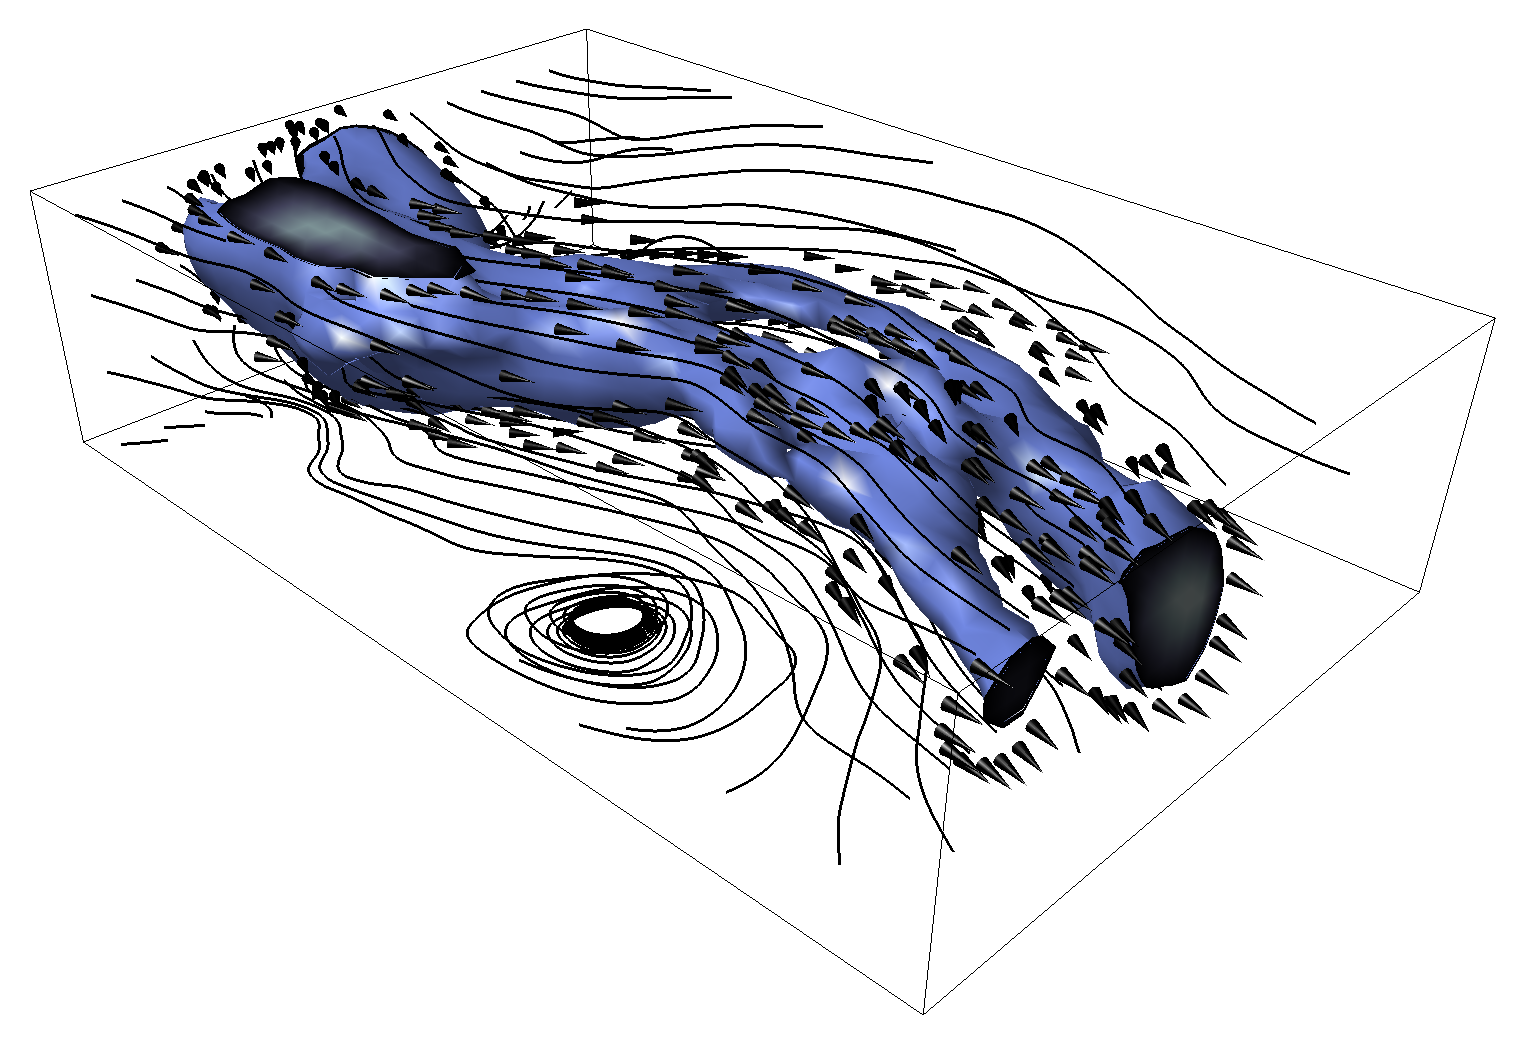
\includegraphics[width=0.9\linewidth]{figure/Wind.png}
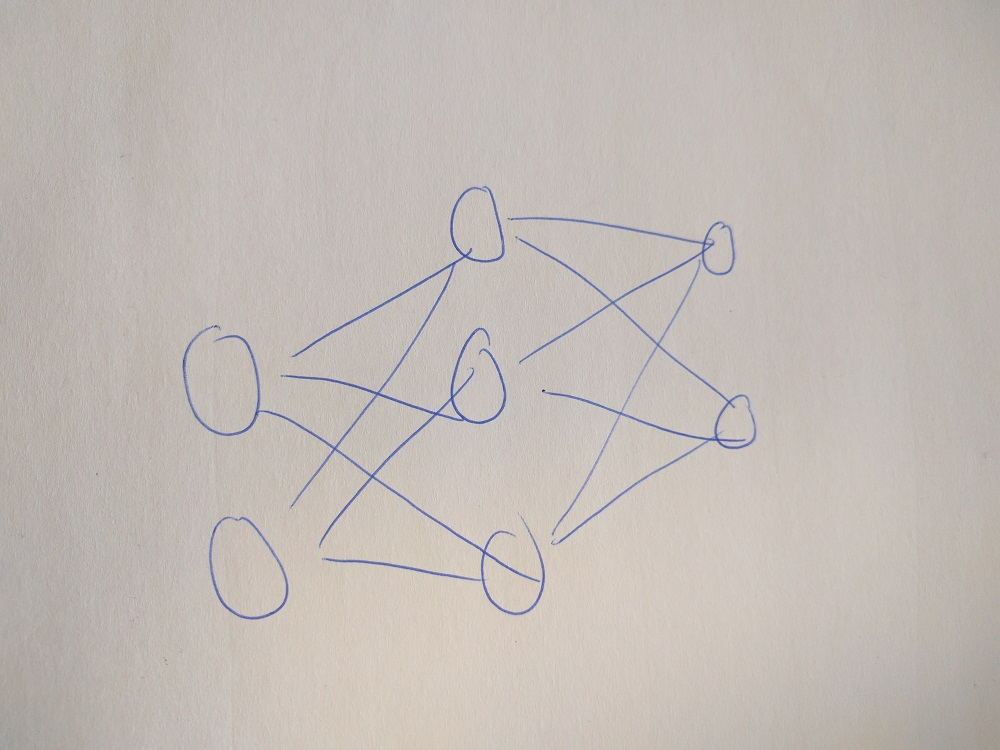
\includegraphics[width=0.9\linewidth]{figure/ann/ann}
\end{figure}

% Cover text
\mbox{}
%\vfill
\renewcommand{\familydefault}{\sfdefault} \normalfont % Set cover page font
\begin{flushleft}
\textbf{{\Huge \varthetitle}} 	\\[0.5cm]
{\LARGE \varthesubtitle}\\[0.2cm]
Bachelor of Science Thesis in Computer Science and Engineering \setlength{\parskip}{0.5cm}

{ JESPER JAXING, ALEXANDER HÅKANSSON, MAXIM GORETSKYY, GMAL TCHAEFA, AXEL OLIVECRONA, JONATAN ALMÉN} \setlength{\parskip}{1.9cm}\\
\vfill
Chalmers University of Technology \\
University of Gothenburg \\
Department of Computer Science and Engineering \\
Göteborg, Sweden, June 2017

\end{flushleft}
%\renewcommand{\familydefault}{\rmdefault} \normalfont % Reset standard font
\end{titlepage}

%\begin{comment} % Remove comment to get blank page
% BACK OF COVER PAGE (BLANK PAGE)
\newpage
\restoregeometry
\thispagestyle{empty}
\mbox{}
%\end{comment}

% TITLE PAGE
\newpage
\setcounter{page}{1}
\thispagestyle{empty}
\begin{center}
	\large Bachelor of Science Thesis\\[4cm]		% Report number given by department 
	\textbf{\large \varthetitle} \\[0.7cm]
	{\large \varthesubtitle}\\[1cm]
	{\large JESPER JAXING}\\
	{\large ALEXANDER HÅKANSSON} \\
	{\large MAXIM GORETSKYY} \\
	{\large GMAL TCHAEFA } \\
	{\large AXEL OLIVECRONA} \\
	{\large JONATAN ALMÉN} \
	
	\vfill	
	% Logotype on titlepage	
	\begin{figure}[H]
	\centering
	% Remove the following line to remove the titlepage logotype
	%
\includegraphics[width=0.2\pdfpagewidth]{figure/front/logo_eng.pdf} \\	
	\end{figure}	\vspace{5mm}	
	
	Department of Computer Science and Engineering \\
	CHALMERS UNIVERSITY OF TECHNOLOGY \\
	University of Gothenburg \\[0.5cm]
	Göteborg, Sweden 2017 \\
\end{center}


% IMPRINT PAGE (BACK OF TITLE PAGE)
\newpage
\thispagestyle{plain}
%\vspace*{4.5cm}
\textbf{\varthetitle}\\
\varthesubtitle
\vspace*{0.5cm}\\
JESPER JAXING\\
ALEXANDER HÅKANSSON\\
MAXIM GORETSKYY\\
GMAL TCHAEFA\\
AXEL OLIVECRONA\\
JONATAN ALMÉN\setlength{\parskip}{0.7cm}

\copyright ~ JESPER JAXING, 2017\\
\copyright ~ ALEXANDER HÅKANSSON, 2017\\
\copyright ~ MAXIM GORETSKYY, 2017\\
\copyright ~ GMAL TCHAEFA, 2017\\
\copyright ~ AXEL OLIVECRONA, 2017\\
\copyright ~ JONATAN ALMÉN, 2017 \setlength{\parskip}{0.5cm}

\todo{Dubbelkolla så detta stämmer}
Examiner: Richard Johansson, Department of Computer Science and Engineering \setlength{\parskip}{1cm}

Department of Computer Science and Engineering\\
Chalmers University of Technology\\
University of Gotehnburg\\
SE-412 96 Göteborg\\
Sweden\\
Telephone: +46 (0)31 772 1000 \setlength{\parskip}{0.5cm}

\vfill
The Authors grants to Chalmers University of Technology and University of Gothenburg the non-exclusive right to publish the Work electronically and in a non-commercial purpose make it accessible on the Internet.\\\\
The Author warrants that he/she is the author to the Work, and warrants that the Work does not contain text, pictures or other material that violates copyright law.\\\\
The Author shall, when transferring the rights of the Work to a third party (for example a publisher or a company), acknowledge the third party about this agreement. If the Author has signed a copyright agreement with a third party regarding the Work, the Author warrants hereby that he/she has obtained any necessary permission from this third party to let Chalmers University of Technology and University of Gothenburg  store the Work electronically and make it accessible on the Internet.


\vfill
% Caption for cover page figure if used, possibly with reference to further information in the report
Cover:\\
A graph visualisation of a simple artificial neural network. See Chapter \ref{chap:ann} for more details. \setlength{\parskip}{0.5cm}

Department of Computer Science and Engineering\\
Göteborg, Sweden 2017


 

% ABSTRACT
\newpage
% CREATED BY DAVID FRISK, 2016
% MODIFIED BY ALEXANDER HÅKANSSON, 2017
\large
\textbf{\varthetitle}\\
\varthesubtitle\\[0.7cm]
JESPER JAXING\\
ALEXANDER HÅKANSSON\\
MAXIM GORETSKYY\\
GMAL TCHAEFA\\
AXEL OLIVECRONA\\
JONATAN ALMÉN\\
\normalsize
\textit{Department of Computer Science and Engineering\\
Chalmers University of Technology\\
University of Gothenburg}\\[0.7cm]
Bachelor of Science Thesis
\setlength{\parskip}{0.5cm}

\thispagestyle{plain}			% Supress header 
\setlength{\parskip}{0pt plus 1.0pt}
\section*{Abstract}
Lorem ipsum dolor sit amet, consectetur adipisicing elit, sed do eiusmod tempor incididunt ut labore et dolore magna aliqua. Ut enim ad minim veniam, quis nostrud exercitation ullamco laboris nisi ut aliquip ex ea commodo consequat. Duis aute irure dolor in reprehenderit in voluptate velit esse cillum dolore eu fugiat nulla pariatur. Excepteur sint occaecat cupidatat non proident, sunt in culpa qui officia deserunt mollit anim id est laborum.

% KEYWORDS (MAXIMUM 10 WORDS)
\vfill
\textbf{Keywords:} lorem, ipsum, dolor, sit, amet, consectetur, adipisicing, elit, sed, do.

\newpage				% Create empty back of side
\thispagestyle{empty}
\mbox{}

% ACKNOWLEDGEMENTS
\newpage
% CREATED BY DAVID FRISK, 2016
\thispagestyle{plain}			% Supress header
\section*{Acknowledgements}
We would like to thank our supervisor Olof Mogren for the great insight and feedback that he has provided during the work with project, making it a fun process and enabling us to succeed. We would also like to thank the division for language and communication for their tremendous help with producing the writing of this thesis. Furthermore, the feedback we have received from other bachelors thesis groups have been of great help.

\newpage				% Create empty back of side
\thispagestyle{empty}
\mbox{}


% TABLE OF CONTENTS
\newpage
\tableofcontents

% OTHER FRONTMATTER
% List of figures (add to table of contents)
\cleardoublepage
\addcontentsline{toc}{chapter}{\listfigurename} 
\listoffigures
% List of tables (add to table of contents)
\cleardoublepage
\addcontentsline{toc}{chapter}{\listtablename}  
\listoftables


% START OF MAIN DOCUMENT
\cleardoublepage
\setcounter{page}{1}
\pagenumbering{arabic}			% Arabic numbering starting from 1 (one)
\setlength{\parskip}{0pt plus 1pt}

\clearpage


%%behövs den här?Känns som en del av theory/dictionary
\begin{comment}
LSTM - Long short term memory
RNN - recurrent neural network
ANN -> Artificial neural network
\end{comment}

%
\makeglossaries
\newglossaryentry{latex}
{
    name=latex,
    description={Is a mark up language specially suited 
    for scientific documents}
}
 
\newglossaryentry{maths}
{
    name=mathematics,
    description={Mathematics is what mathematicians do}
}

\begin{comment} % Känns som acronyms == dictionary, borde välja en av dem? Alla vetenskapliga saker borde vara i teorin såsom ANN.

% acronym är ju mer förkortningar så som ANN, dictionary är ju ordlista förklarar vad ett artfical neural network är.
Artificial neural network -> Mathematical model inspired by biological neural networks (brains)
Learning rate -> parameter that adjust how big of a step is taken towards goal
Baseline -> a criteria for comparison
Deep learning -> a form of an artificial neural network with more than three layers.
Labeled data -> data with known classifications data with known classifications.
Hyperparameters -> parameters manually set to define the structure and rigidity of a neural network
paramater -> A constant number in the model that is updated during training
Softmax  -> function that scales the vector entries to be between 0 and 1, while making them sum to 1
Recurrent neural network -> a form of neural network whose graph can have cycles
Training data -> data used for training the network 
Mentioning and highlighting -> a way of notifying a user.
Tensorflow --> Machine learning library
Overfitting -> Overfitting has occured when the validation error goes up and the traning error goes down. If Overfitting has occured generality has been lost and the model has learnt the training data to well.
\end{comment}

% INTRODUCTION
% CREATED BY DAVID FRISK, 2016
\chapter{Introduction}
This chapter presents the section levels that can be used in the template. 

\section{Section levels}
The following table presents an overview of the section levels that are used in this document. The number of levels that are numbered and included in the table of contents is set in the settings file \texttt{Settings.tex}. The levels are shown in Section \ref{Section_ref}.

\begin{table}[H]
\centering
\begin{tabular}{ll} \hline\hline
Name & Command\\ \hline
Chapter & \textbackslash\texttt{chapter\{\emph{Chapter name}\}}\\
Section & \textbackslash\texttt{section\{\emph{Section name}\}}\\
Subsection & \textbackslash\texttt{subsection\{\emph{Subsection name}\}}\\
Subsubsection & \textbackslash\texttt{subsubsection\{\emph{Subsubsection name}\}}\\
Paragraph & \textbackslash\texttt{paragraph\{\emph{Paragraph name}\}}\\
Subparagraph & \textbackslash\texttt{paragraph\{\emph{Subparagraph name}\}}\\ \hline\hline
\end{tabular}
\end{table}

\section{Section} \label{Section_ref}
\subsection{Subsection}
\subsubsection{Subsubsection}
\paragraph{Paragraph}
\subparagraph{Subparagraph}


%Diskutera datan:(notera det här är bara bajs så vi kan diskutera något senare, därför skriver jag på svenska //maxim)
%Vi kunde få ut X antal interaktioner med trådar på reddit, där en interaktion motsvarar en downvote eller upvote.Varje interaktion är kopplad till en specific person i datasettet. Vi får också ut vilken subreddit tråden var skapad på, och eventuell innehåll(content).
\\ %Den här kan typ vara i terminologi, eftersom vi endast förklarar hur datan ser ut.
%I första modellen tog vi bara ut de "positiva" interaktioner, dvs alla med upvotes, och grupperade datan så att varje titel har ett set av användarna (i postgres). För att träna den första modellen var vi bara intresserade av titeln och användarna, dvs titel var vår inputdata och mängden av användarna var vår "target"/"labeled" data, dvs den outputten som vi vill att den ska få. 
%tl;dr input = titel, output = användarna som är intresserade.
%En annan ide är att även använda de negativa interaktioner(downvotes), man kan tolka det på olika sätt: en downvote kan vara att du är inte intresserad av det och då borde man straffa modellen mer om en användare ger en downvote på en titel, det andra sättet och tolka är på är att man är intresserad men håller inte med personen eller tycker inte om sättet någon beskrev det på, men själva ämnet är fortfarande intressant. Det leder till två olika modeller/approaches som man kan undersöka.
\newpage
\chapter{Artificial Neural Networks}\label{chap:ann}
This chapter will discuss the basics of artificial neural networks (ANNs) which will be referenced throughout the rest of the thesis. All the techniques and theory discussed in this chapter have been used in some way to achieve the results presented in chapter \ref{chap:results}. This chapter will not introduce anything new to someone who is familiar with ANN.

\section{Introduction to Artificial Neural Networks}
An artificial neural network is a machine learning model inspired by biological neural networks \parencite{lippmann1987introduction}. \cite{Goodfellow-et-al-2016} describe an ANN as a directed and acyclic graph (see figure \ref{fig:simple_ann}). They go on to say that the network is constructed of artificial neurons which are structured in layers -- these neurons are represented as nodes in a graph. Each neuron represents a function that takes some input from other nodes and produces an output. The input data to the network is represented by a vector $\vec{x} = [x_1, x_2, x_3, \dots, x_n]^T$ with $n$ features. The vector $\vec{x}$ could for example represent a whole sentence where $x_i$ represents a word.
\\\\
The edges in the network are connections between pairs of neurons. Each connection between two neurons have a weight. These weights will change as the network is optimised, as described in section \ref{sec:trainingoptimisation}, and the way they change will directly change the network's output. Updating the weights between neurons is a key part of how an ANN works, as the connections directly affect the output of the network. In practice this means that the weights should be updated so that the network gradually produces an output more similar to the desired target. 
\\\\
The input to a layer is the matrix product between the output from a previous layer and the weights between those two layers (usually with some bias term added as well). The weights are used to transform the input before it is propagated to subsequent layers. A convenient way to represent weights between two layers $j$ and $k$ is by a matrix, $W_{jk}$, where each element is the weight between a neuron in layer $k$ and a neuron in layer $j$, where $k<j$. Let $\vec{z_j}$ denote the input to layer $j$ where $W_{jk}$ are weights to layer $j$ from layer $k$ and $\vec{x_k}$ is the output from layer $k$. The vector $\vec{b}$ is a bias term that is added for more degrees of freedom. 
\begin{equation}\label{eq:z}
    \vec{z_j} = \vec{W_{jk}} \cdot \vec{x_k} + \vec{b_j}
\end{equation}
Let $\vec{y_i}$ denote the output of the layer $i$. For the first layer (input layer) $\vec{y_1}=\vec{x}$. The output, $\vec{y_i}$, of a layer $i$ is the result of applying some activation function on $\vec{z_i}$ as shown in equation \ref{eq:f_of_z}. Activation functions are described in further detail in section \ref{activationfunction} but can in summary be seen as a way to scale the output element wise.
\begin{equation}\label{eq:f_of_z}
    \vec{y}_i = f(\vec{z}_i)
\end{equation}
During training, once the data have been propagated to the last layer, an error function will be used to measure the error of the model by comparing the final output/prediction with the expected output for the given input. The details about error functions can be found in section \ref{errorfunction}. Furthermore, the results of the error functions are used when training the network, which is explained in section \ref{sec:trainingoptimisation}. 
\\\\
Depth and width are often used to describe the shape of an artificial neural network \parencite{Goodfellow-et-al-2016}. The depth determines how many layers the network contains. The layers between input and output layer are called hidden layers. The more neurons a layer has the wider it is considered. \parencite{Goodfellow-et-al-2016} states that the reason for using multiple layers are taken from research in neuroscience. A large network (in either dimension) has more degrees of freedom which generally means that it will fit the data better, but will possibly overfit (see section \ref{sec:overfitting}).

\begin{figure}[h]
    \centering
    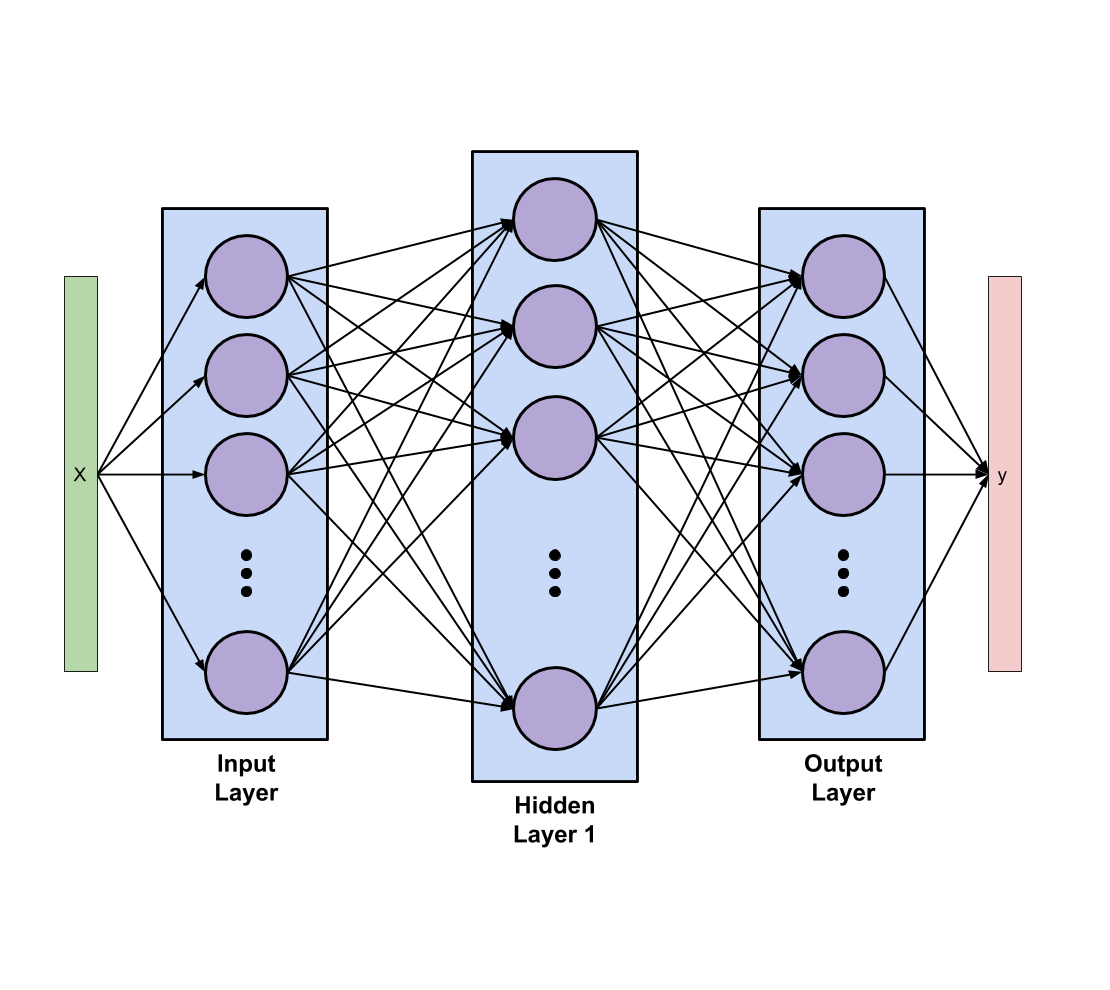
\includegraphics[width=0.75\textwidth]{figure/ann/simple_ann}
    \caption{A graph visualisation of a simple ANN. $\vec{x}$ and $\vec{y}$ are input and output vectors respectively}
    \label{fig:simple_ann}
\end{figure}

\section{Uses of Artificial Neural Networks}
A common use of machine learning is classification. It is the task of classifying a given data point as belonging to one (or more) of $k$ sets based of previously observed data \parencite{Michie94machinelearning}. Classification can be visualised as a graph of data points with a curve separating the $k$ sets, this curve is also referred to as decision boundary. For the purpose of this project an artificial neural network will be used for classifying content to users. There are however a lot of different machine learning techniques which solves the problem of automatically classifying data, e.g. Naïve Bayes Classifier \parencite{rish2001empirical}, Support Vector Machines (SVM) \parencite{boser1992training, cortes1995support}, or Decision Tree Classifier \parencite{safavian1991survey}.
\\\\
Classification of data typically requires extraction of features that can be compared - feature engineering, as this is called, is a process that usually requires extensive domain knowledge. When using artificial neural networks, the process of feature engineering can be omitted  thus making it easier to model more complex problems \parencite{nlp2011ronan, lecun2015deep}. This property of artificial neural networks makes them suitable for many tasks, among others to model sequences of text as it is not necessary to manually find features in the text that could be used for classification, which motivates their usage for this project.


\section{Activation Functions}\label{activationfunction}
The activation function scales the output from a node to create a new signal that is sent to the next layer \parencite{basheer2000artificial}. By using non-linear functions it is possible to scale the output, and find non-linear decision boundaries which allow better fitting to the data \parencite{lippmann1987introduction, basheer2000artificial}. Different activation functions can be used for different purposes in the same artificial neural network, it is not necessary to choose only one. In this project a few different activation functions have been used, and are described below.

\subsection{Logistic Function}\label{sec:sigmoid_function}
The logistic function is a non-linear function with a \textit{S} shaped curve defined by equation \ref{eq:sigmoid} that squashes the input, $z_j$ from equation \ref{eq:z}, between $[0, 1]$.
\begin{equation}\label{eq:sigmoid}
    f(\vec{x})=\frac{1}{1+exp(\vec{-x})}
\end{equation}
For this project the logistic function has been used in the final layer as the output function as it is possible to interpret its output as probabilities. This particular function is especially useful for multi-label classifications (where some input can be classified as belonging to more than one class, like the problem presented in this thesis). When using the logistic function like this it is common to use the negative log-likelihood error function as this is particularly useful for multi-label classifications \parencite{bishop1995neural}.

\subsection{Rectified Linear Unit Function}\label{sec:relu}
The Rectified Linear Unit (ReLU) function is a non-linear function defined by equation \ref{eq:ReLU}. This function has the benefit of being unbounded as opposed to the logistic function, the range of which is the interval $[0, 1]$. The ReLU function has become popular in the past few years due to it being less susceptible to vanishing gradient compared to other activation functions \parencite{glorot2011deep, lecun2015deep}.
\begin{equation}\label{eq:ReLU}
    f(x) = max(0,x)
\end{equation}
The ReLU function was used as the activation function in the hidden layers.

\subsection{Softmax Function}\label{sec:softmax_function}
The softmax function is defined by equation \ref{eq:softmax} where $\vec{x}$ is a vector of $n$ outputs. Softmax scales the vector entries to be between $[0,1]$, while normalising them all to sum to 1.
\begin{equation} \label{eq:softmax}
    f(x_j) = \frac{e^{\vec{x}_j}}{\sum_{i=1}^{n} e^{\vec{x}_i}}
\end{equation}
When using the softmax function in the final layer of the network to create an output it has been shown that the cross entropy error function gives a better accuracy compared to others \parencite{dunne1997pairing,golik2013cross}. By using the softmax activation function the output can be interpreted as normalised probabilities between the $n$ output classes. Because of the normalisation this becomes useful for classification where there is only one correct true class. Softmax is used during pretraining of the network, when it is trained to predict exactly one subreddit. (see section \ref{sect:enhacing_the_model})

\section{Error Functions} \label{errorfunction}
The error functions in neural networks are used to compare the network's predicted output with the correct output for a given input. This is used when training the network by using the comparison to minimise the error, more details in section \ref{sec:trainingoptimisation}. There are primarily two different error functions that are used and evaluated in this project. In these sections $y_k$ indicates the $k^{th}$ prediction of the network, $t_k$ indicates the target value of the $k^{th}$ class, and $K$ is the number of classes.
\\\\
One of the error functions examined is the Cross Entropy error function. The function is very commonly used when working with ANN because of its overall performance, compared to alternatives, when performing backpropagation (see section \ref{sec:backpropagation} for details on backpropagation). The cross entropy function is defined as in equation \ref{eq:cross_entropy} \parencite{bishop2006crossEn}.
\begin{equation} \label{eq:cross_entropy}
    E_K = -\sum_{k=1}^{K} [t_k \cdot ln(y_k) +(1-t_k)ln(1-y_k) ]
\end{equation}
The reason behind its popularity is that the derivative with respect to the weights is proportional to the difference between the predicted value and actual value, leading to better performance of the network due to a lower stagnation period \parencite{nasr2002cross}.
\\\\
The other error function that is evaluated is the Negative Log-Likelihood (sometimes called Multi-Class Cross Entropy) function \parencite{bishop2006pattern}. This error function, defined in Equation \ref{eq:neg_log_likelihood} \parencite{tensorflow2016cross}, could be interpreted as a more general version of the Cross Entropy function. It is more suitable for multi-label classification problems compared to the Cross Entropy function which is suitable for single-label classifications.
\begin{equation} \label{eq:neg_log_likelihood}
    E_K = \vec{t} -log(\vec{y}) + (1-\vec{t}) -log(1-\vec{y})
\end{equation}
In this project the Negative Log-Likelihood function is used as the error function when using the logistic function (see equation \ref{eq:sigmoid}) as output function for the network.

\section{Training and Optimisation} \label{sec:trainingoptimisation}
Training and optimisation in machine learning is the process of learning from data. The way a certain machine learning technique learns from data usually differs but the training of an artificial neural network can be seen as a problem of optimising the network's weights. For this to work an error function is needed that determines how much a certain prediction for a data point is wrong compared to the true classification of that data point. The optimisation objective is to find the weights and biases in the artificial neural network that minimises the error for the training data. This can be achieved by applying backpropagation and some optimisation method, e.g. Gradient descent (see section \ref{sec:gradient_descent}). The process of learning from some previously classified data is called supervised learning \parencite{lecun2015deep}. This training process is required to improve the performance of  the artificial neural network. \parencite{Goodfellow-et-al-2016}.

\subsection{Gradient Descent Optimisation}\label{sec:gradient_descent}
Gradient descent is an iterative algorithm where the gradient of a function is calculated in steps. The computed gradient is used to move towards the minimum of the function. This is repeated until a local or global minimum of the function is found. Computing the gradient for the whole dataset is computationally heavy. This together with the fact that the return is less than linear in batch size \parencite{Goodfellow-et-al-2016} leads to that the datasets used for training are divided into small batches, minibatches, because of computational limitations when processing the whole dataset. When using minibatches, the gradients of the error function for each datapoint in the minibatch is computed and then averaged to approximate the full gradient. When applying gradient descent to this approximation it is known as Stochastic Gradient Descent (SGD). It has been shown that SGD has a good running time for convex functions \parencite{convexSGD}. There are no guarantees that an artificial neural network will be convex, however there is a specialised and efficient implementation of gradient descent called \textit{Adam} \parencite{adamoptimizer} that is commonly used for artificial neural networks. The Adam optimiser is used in this project to optimise the weights and biases of the ANN model to give a minimal error. By minimising the error the predictions of the network should improve, if the model is working.

\subsection{Using Backpropagation}\label{sec:backpropagation}
Backpropagation is a method used for training artificial neural networks. When you feed an input vector (a sentence for example) to the network. The network will propagate the vector forward until it reaches the last layer and presents a result/prediction. The prediction is then compared to the desired result for the given input via an error function to determine how well the network performed. The error is then propagated backwards through the network to determine how much every individual weight affected it. The weights and biases for each neuron is then updated accordingly. How the weights and biases are updated depends on what optimisation method is used. This training is performed on all of the data points in a training data set and each training iteration over a complete set is called an epoch.

\subsection{Overfitting}\label{sec:overfitting}
Overfitting can be described by a state of the model where the network does not generalise too well, meaning that the network is too accustomed to the training data and its details. This phenomenon results in bad accuracy of the network on the unseen data. This is a common problem if the network has too many parameters that can describe the training data instead of capturing the general idea of the data.
\begin{figure}[h]
    \centering
    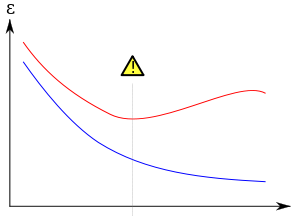
\includegraphics[width=0.5\textwidth]{figure/ann/overfitting}
    \caption{A toy example of overfitting. The red line shows the error on the validation data and the blue line shows the error on the training data. It is desired that the error is as low as possible. 
    "\href{https://en.wikipedia.org/wiki/Overfitting\#/media/File:Overfitting_svg.svg}{Overfitting}" by
    \href{https://commons.wikimedia.org/wiki/User:Gringer}{Gringer} edited by
    \href{https://commons.wikimedia.org/wiki/User\:Dake}{Dake} is licensed under CC-BY 3.0.}
    \label{fig:overfitting}
\end{figure}
\\
As seen in Figure \ref{fig:overfitting} the network is performing better and better for both training and validation sets. However, it reaches a point where the validation error starts going up. That point is where the overfitting has occurred. The training error is still decreasing meaning that the network keeps learning on the training data instead of generalising from it. 

\subsection{Regularisation}\label{sec:regularisation}
Regularisation is a set of techniques used in order to prevent the overfitting problem described in section \ref{sec:overfitting}. These techniques increase the performance of the network as it can continue to generalise without overfitting. 
In this thesis two different regularisation techniques have been used:
\begin{itemize}
    \item Dropout
    \item $l^2$-loss regularisation
\end{itemize}
These will be explained below.
\\\\
Dropout is a rather newly discovered regularisation technique that prevents overfitting by randomly disabling neurons in the ANN \parencite{srivastava2014dropout}. During the training of the network, neurons are randomly disabled with a probability $p$. This means that the network has to teach other neurons to do the generalisation that the disabled neuron previously did. It is important to note that this is only used during the training of the network. When validating the performance of the network or actually using the network all neurons are used.
\\\\
The purpose of $l^2$-loss regularisation is to prevent weights from becoming extremely large by penalising them based on how large they are. The $l^2$ regularisation is used by adding the $l^2$-norm of every weight in the ANN to the error function. The penalisation leads to a limitation in the network's capacity, or \textit{statistical complexity}, in terms of the $l^2$-norm \parencite{neyshabur2015norm}. 
\\\\
A powerful aspect of these two regularisation techniques is that they work alongside each other. This is because they are implemented in different parts of the ANN model.

\section{Recurrent Neural Networks }\label{sec:rnn}
A recurrent neural network (RNN) is an artificial neural network that takes context into account. It accounts for context in the sense that the current output is dependent on the previous. This context dependency is often depicted as an ANN that has its own output as input, in practice however RNNs are instead modelled as chained (or \textit{unfolded}) \textit{units} as shown in Figure \ref{fig:chained_units}. A unit takes two inputs; the output from the previous unit and input data. The output produced is passed along to the next unit but could also be retrieved and used. An arbitrary number of units can be chained in this way but in this project the number of units will be related to the length of the input text. 
\begin{figure}[h!]
    \centering
    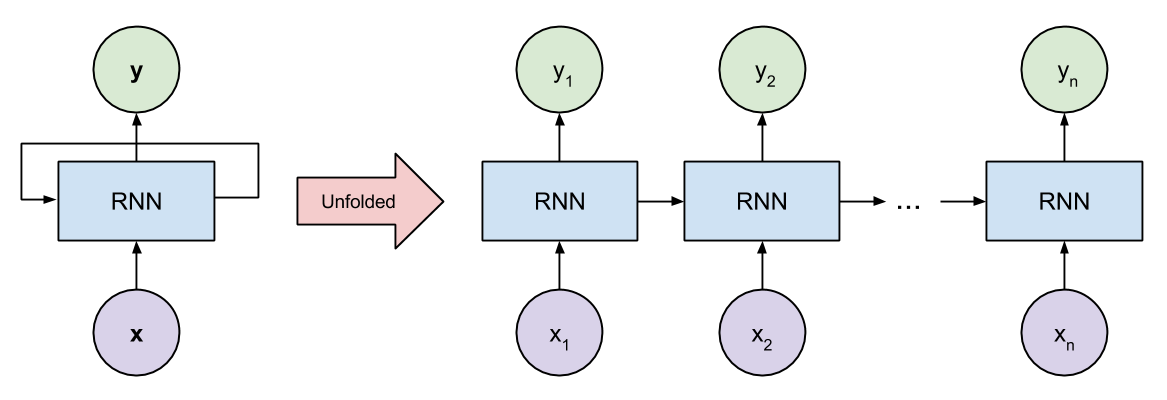
\includegraphics[width=0.95\textwidth]{figure/ann/rnn_unfold}
    \caption{A visualisation of a recurrent neural network layer and how it is unfolded. $\vec{x}$ and $\vec{y}$ are the input and output vector respectively}
    \label{fig:chained_units}
\end{figure}
\\\\
RNNs are particularly useful when modelling with natural language as input since words in a sentence often are dependent on what comes before them. When using sentences as input to a RNN, it is common to have each word as an input to one unit in the RNN \parencite{palangi2016deep}. This is how RNNs will be used in this project to model social platform content.
\\\\
The units in a recurrent neural network can be implemented in different ways. Popular unit implementations are Long Short Term Memory (LSTM) and Gated Recurrent Unit (GRU). The LSTM unit was introduced to solve the problems of inefficiency in the backpropagation for RNNs \parencite{LSTMdefined}. The inefficiencies occurred because the error gradient would decay and approach zero, making training very slow, and this is what the LSTM solves \parencite{hochreiter1998vanishing}. The GRU is a fairly recent addition to the field of RNN. It performs similarly to the LSTM and the dataset used can have a big impact on which one performs better \parencite{GRUchung2014empirical}. The fact that either of the unit implementations might perform better based on the dataset used motivates testing them both in this project.

\subsection{Using Recurrent Neural Networks for Natural Language Processing}\label{sec:rnn_nlp}
As previously mentioned, when working with natural language it is common to let every unit in a RNN layer take one word as input. This is illustrated in figure \ref{fig:sentence_to_rnn} below.
\begin{figure}[h]
    \centering
    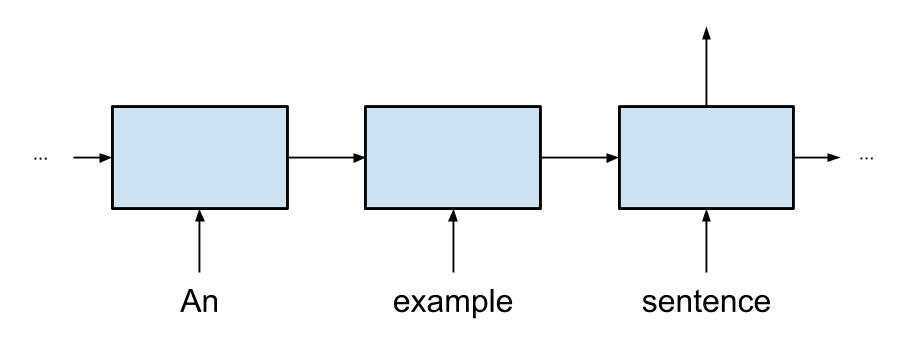
\includegraphics[width=0.75\textwidth]{figure/ann/sentence_to_rnn}
    \caption{A simplification of how a recurrent neural network layers process natural language as input}
    \label{fig:sentence_to_rnn}
\end{figure}
\\
However, RNN units, just as an ANN, expect some vector. This means that the input sentences have to be vectorised. A common way to achieve this is to use indices instead. With this approach each unique word is given a unique number, and an input sentence of words then become a vector of word indices. It is also common to take the transformation one step further and turn each word index into a so called one-hot vector \parencite{turian2010word}. Using one-hot vectors, each word is represented as a vector $\vec{w}$ of length $C$, where $C$ represents the total number of words, having a $1$ at the position of the given word's index and zeros everywhere else, this is illustrated by the table \ref{tab:onehot}. Since the length of the vector is fixed, it means that the new words that are not in the dictionary can not be represented as a one-hot vector. 
\begin{table}[h]
    \centering
    \begin{tabular}{c|c|c|c|c}
    This & is & a & normal & sentence\\
    \hline
    1 & 0 & 0 & 0 & 0\\
    0 & 1 & 0 & 0 & 0\\
    0 & 0 & 1 & 0 & 0\\
    0 & 0 & 0 & 1 & 0\\
    0 & 0 & 0 & 0 & 1
    \end{tabular}
    \caption{An illustration of how the sentence "This is a normal sentence" as one-hot vectors, given that the vocabulary is \{a, is, normal, sentence, this\}}
    \label{tab:onehot}
\end{table} 
\\\\
Another problem with one-hot vectors is that they do not hold any information about relationships between words. This motivates using another representation for words in order to capture the connection. This can be done with algorithms such as word2vec \parencite{mikolov2013linguistic} or GloVe \parencite{pennington2014glove}. 
\newpage
\chapter{Method}%Är metod och utförande samma sak?
This chapter will describe the workprocess of this project and what has been done.
\section{Deciding on a dataset}
måste vara naturligt labeled
\subsection{Ubuntu dialogue corpus}
This data set consists of back and forth conversations between users. Even thought the dataset is large it is not natural labeled for our needs and it is not clear how training on back and forth conversations would help it prediction what users would find a post on the web interesting. The Ubuntu dialogue corpus was ultimately not used since the data was not suited to our task.
\subsection{Reddit}
\section{Gathering data}
något om att deep ann:s behöver mycket data %Must be mentioned in theory part
\section{Modeling as an RNN}
\subsection{Tensorflow}%The explanation about tensorflow should be made in terminology, here we shall only name how we will use it.
Tensorflow is a high level framework, developed by Google to give the possibility of developing machine learning applications without having a deep knowledge. %även om det är sant att man inte behöver vara ML proffs tycker jag det får oss att låta dumma% 
\subsection{LSTM-network}
\subsection{Scaling down}
As by suggestion from our supervisor we will begin with a very small scale network, instead of having the number of users in the tens of thousands we will start with 2-5 users. The reasoning for this is it that it will now be easier to not just train the network but to also to analyse it. This is a common approach in machine learning (source Olof) and the hope is that whatever model works on the small scale will hopefully continue to perform when it is scaled up.    
\subsection{Overfitting on purpose}
Overfitting is something you want to avoid in the final model but can be useful in development. Overfitting is a result of having learnt the training data too well but the key here is that something has been learnt. If the model has learnt something you at least know you are on the right path, it is not making guesses at random. Overfitting is therefore the first milestone for our scaled down network. 
\subsection{Scaling up}
\subsection{Tuning hyperparameters}
\section{Baseline}
When deciding how well a model performs it is compared against a baseline. The baseline puts the accuracy of the model into some context. You might have an accuracy of 90\%, is that good or bad? You need one or more baselines to decide this. 
\subsection{Random classifier}
A random classifier is a model that given an input $x$ selects one of $n$ output values uniformly at random. This results in an expected accuracy of $\frac{1}{n}$. This is a baseline that any real life model needs to beat with confidence.
\subsection{Collaborative filtering}
%Flytta förklaringen till ordlista? 
Collaborative filtering can be used in what is called recommender systems. The goal of a recommender system is to recommend users products that the user finds interesting or helpful. Collaborative filtering operates under the assumption that if Bob likes cats and dogs and Alice likes cats, Alice is more likely to also like dogs since Bob likes dogs and Alice share a interest with Bob. Collabortive filtering has found success in recommending items such as movies (netflix prize source). %Kanske något mer om hur vi använde detta som baseline%

\subsection{N-gram}
\section{Computing power restrictions} %Should 
\section{Integration with an application}


%Saker som man är också intressanta: Kolla upp variansen, debugg, hur vi hitta felet etc. 
\newpage
\chapter{Results}\label{chap:results}
This chapter will present the results achieved in the project as described in Chapter \ref{chap:method}. These results includes comparisons between different models and their hyperparameters but also a look at the different datasets that were used.

\section{Analysis of the datasets}
\label{sec:dataset-summary}
The purpose of this section is to present the result of an investigation into the different datasets. The goal of this was to see if there were any irregularities or patterns in the datasets that could have had an affect on the performance of the networks or the baselines. 
\subsection{5 user data set allvotes}
\label{sec:five-user-data-set}

One thing that we found in the training set for the five user dataset was that the difference in length of the longest title and the second longest title was large. The longest title was 1928 words while the second longest was 66 words. This skewed the variance for the training data and is why one standard deviation sits at $24.9$ as you can see in \ref{table:5-user-set-train} while all the other datasets sits around $10$. If the outlier is removed, one standard deviation is brought down to $9.7$ and sits around the same value as all the other.
\\\\
Another point of interest is how few users share liked titles. In the training set \ref{table:5-user-set-train} you can see that only about $1\%$ of titles have more than 1 up or downvote. In the validation \ref{table:5-user-set-train} and test set \ref{table:5-user-set-train} it is even less titles, $0.45\%$ for the validation and $0.6\%$ for the test set.
\\\\
The data regarding the vote density in subreddits for the $50$ users datasets have been left out simply due to the size of the tables they would require, the data is however available in appendix \ref{appendix:dataset} if the reader is interested.


\begin{table}[H]
    \centering
    \begin{tabular}{ r | c | c | p{4cm}  }
    \hline
    \textbf{User} & \textbf{Active subreddits} & \textbf{Total votes} & \textbf{Votes in two most voted subreddits} \\ \hline \hline
    \multicolumn{4}{c}{\textbf{Training data set}} \\ \hline \hline
    Ayavaron & 64 & 1411 & 444 \\ \hline
    akkartik & 14  & 1387 & 1333 \\ \hline
    crmaki & 14 & 1410 & 902 \\ \hline
    izzycat & 37 & 1363 & 505 \\ \hline
    doctorgonzo & 32 & 1429 & 586 \\ \hline \hline
    \multicolumn{4}{c}{\textbf{Validation data set}} \\ \hline \hline
    Ayavaron & 40 & 416 & 133 \\ \hline
    akkartik & 8  & 392 & 372 \\ \hline
    crmaki & 11 & 390 & 252 \\ \hline
    izzycat & 26 & 428 & 158 \\ \hline
    doctorgonzo & 24 & 364 & 146 \\ \hline \hline
    \multicolumn{4}{c}{\textbf{Testing data set}} \\ \hline \hline
    Ayavaron & 33 & 172 & 60 \\ \hline
    akkartik & 5  & 220 & 212 \\ \hline
    crmaki & 12 & 194 & 131 \\ \hline
    izzycat & 19 & 207 & 77 \\ \hline
    doctorgonzo & 28 & 204 & 78 \\ \hline
    \end{tabular}
    \caption{Vote distribution for the training, validation and testing data sets with five users}
    \label{table:5_user_reddit_dataset}
\end{table}
\todo{Dubbel kolla siffrorna}
\begin{table}[H]
    \centering
    \begin{tabular}{ r | c | c | c }
    \hline
    \textbf{Feature} & \textbf{Training} & \textbf{Validation} & \textbf{Testing} \\ \hline \hline
    \multicolumn{4}{c}{\textbf{Titles}} \\ \hline \hline
    Amount & 6927 & 1983 & 992 \\ \hline
    Median length & 9 & 9 & 8 \\ \hline
    Average length & 12 & 11 & 11  \\ \hline
    Within $\sigma$ title length & 24.9 & 9.6 & 9.4 \\ \hline
    Longer than average & 2198 & 696 & 320 \\ \hline
    More than 1 vote & 76 & 9 & 6 \\ \hline
    More than 2 votes & 2 & 0 & 0\\ \hline \hline
    \multicolumn{4}{c}{\textbf{Subreddits}} \\ \hline \hline
    Amount & 103 & 65 & 59  \\ \hline
    Average voted in in & 32.2 & 21.8 & 19.4 \\ \hline
    Within $\sigma$ voted in & 18.4 & 11.49 & 10.2  \\ \hline
    \end{tabular}
    \caption{Statistics for the dataset containing five users}
    \label{table:5-user-set-train}
\end{table}
\subsection{50 user data set allvotes}
Here there are not any big outliers in title length as in the five user dataset but there is a higher percentage of users that share liked titles compared to the five user dataset. In the training set for the fifty user dataset, $7.75\%$ of titles have more than one up or downvote. In the validation set it is $6\%$ and for the testing set it is $5.7\%$.


\begin{table}[H]
    \centering
    \begin{tabular}{ r | c | c | c }
    \hline
    \textbf{Feature} & \textbf{Training} & \textbf{Validation} & \textbf{Testing} \\ \hline \hline
    \multicolumn{4}{c}{\textbf{Titles}} \\ \hline \hline
    Amount & 63176 & 18486 & 9301 \\ \hline
    Median length & 9 & 9 & 9 \\ \hline
    Average length & 12 & 12 & 12  \\ \hline
    Within $\sigma$ title length & 11.7 & 9.3 & 9.3 \\ \hline
    Longer than average & 23474 & 6736 & 3354 \\ \hline
    More than 1 vote & 5428 & 1231 & 577 \\ \hline
    More than 2 votes & 980 & 220 & 92\\ \hline \hline
    \multicolumn{4}{c}{\textbf{Subreddits}} \\ \hline \hline
    Amount & 343 & 248 & 192  \\ \hline
    Average voted in in & 31.28 & 22.6 & 18.58 \\ \hline
    Within $\sigma$ voted in & 17.6 & 12.17 & 9.88  \\ \hline
    \end{tabular}
    \caption{Statistics for the dataset containing fifty users}
    \label{table:50-user-set-train}
\end{table}

\todo{moar plots/graphs}

As seen in figure \ref{fig:histvotes} most of the posts have a low number of upvotes, this could potentially mean that it is hard to learn from this data.

\begin{figure}[H]
    \centering
    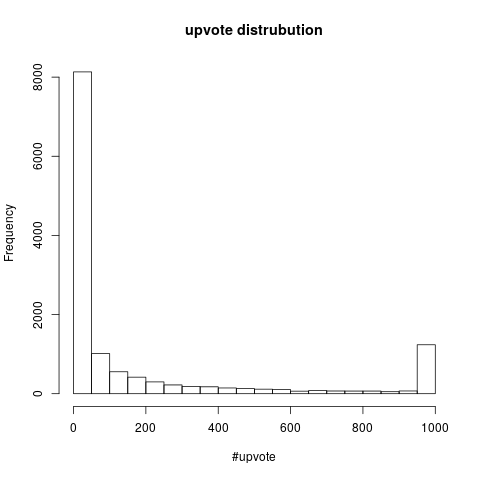
\includegraphics[width=0.75\textwidth]{figure/results/histupvote}
    \caption{A histogram with number of upvote per post on the x axis and number of posts on the y axis.}
    \label{fig:histvotes}
\end{figure}


\section{The first iteration model}
The first iteration of the model was implemented with no hidden layers, as described in section \ref{sec:modelling_the_ann}. It had an LSTM-RNN layer as its input layer with 30 LSTM units. Full details on this model are found in section \ref{sec:app2_first_iter}. When this model was trained on a dataset downscaled to contain five users overfitting was achieved as shown in figure \ref{fig:first_iter_overfitting}.
\begin{figure}[h!]
\begin{subfigure}{0.5\textwidth}
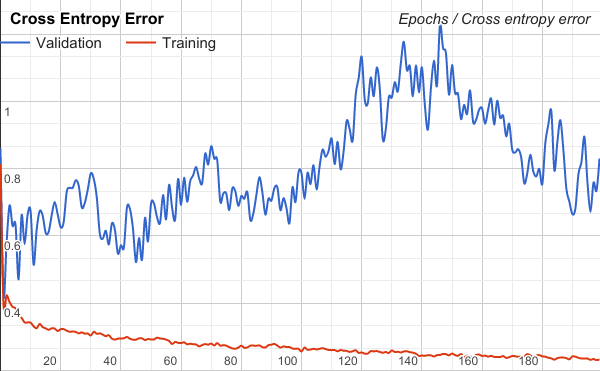
\includegraphics[width=1 \linewidth]{figure/results/first_iter_cross}
\caption{Cross entropy error}
\label{fig:first_iter_overfitting}
\end{subfigure}
\begin{subfigure}{0.5\textwidth}
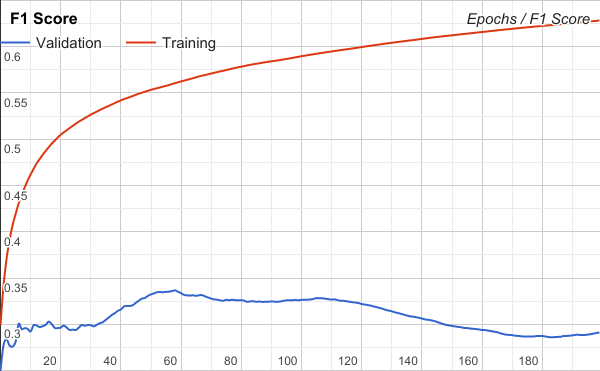
\includegraphics[width=1\linewidth]{figure/results/first_iter_f1}
\caption{$F_1$ score.}
\label{fig:first_iter_f1}
\end{subfigure}
 
\caption{The cross entropy error and $F_1$ score of the first iteration model after 200 training epochs, trained on the training and validation sets. It is good to achieve a low error and a high $F_1$. $F_1$ ranges between $0$ and $1$ inclusive.}
\label{fig:image2}
\end{figure}
\\
The best $F_1$ score achieved on the validation set using the model was $0.3366$, as shown in figure \ref{fig:first_iter_f1}, but the main takeaway was that the model is able to learn from the data.

\section{The final network}
The most optimal network we managed to achieve for the five user dataset had an accuracy of about $39\%$. Even after 1470 epochs this model had not overfitted, however the performance hardly got better after more epochs.

\subsection{Hyperparamaters}
The final result of the hyperparamaters are shown in table \ref{table:hyperparameters_final}

\begin{table}[h!]
    \centering
    \begin{tabular}{ r  p{7cm} }
        \hline
        \textbf{Hyperparamter}  &  \textbf{Value} \\ \hline \hline
        Learning rate & $0.05$  \\ \hline
        Batch Size & $25$ \\ \hline
        RNN units & $400$  \\ \hline
        Embedding Size & t $300$ \\ \hline
        Pre-trained embedding matrix & $False$ \\ \hline
        Trainable embedding matrix & $True$ \\ \hline
        Hidden layers & $1$ \\ \hline
        Neurons in hidden layers & $300$ \\ \hline
        Use L2 regularisation & $True$ \\ \hline
        L2 Factor & $0.01$ \\ \hline
        Dropout regularisation & $True$\\ \hline
        Dropout probability & $0.75$ \\ \hline
        Use constant prediction limit & $False$ \\ \hline
        Constant prediction limit & N/A  \\ \hline
        Use subreddit input & $False$ \\ \hline
    \end{tabular}
    \caption{Final value for all hyperparamaters}
    \label{table:hyperparameters_final}
\end{table}
\section{Baseline comparison} 
\todo{lägga in fina tabeller}
\subsection{Facebook fastText classifier}

\subsection{Random classifier}

\subsection{N-grams}
The F1-score of $0.3898$ was achieved with n-grams when performing on the dataset with five users.
\todo{kör testet med 50 användare sen, GLÖM INTE PLSPLSPLSPLSPLSPLS}


\newpage
\chapter{Discussion}\label{chap:discussion}

This chapter will discuss the obtained results from Chapter \ref{chap:results} and potential problems with the methodology leading to them.

\section{The Models and Their Performance on the Datasets}
The best performing network, as seen in Section \ref{sec:final_model}, got an $F_1$ score of $0.4548$ on the five users dataset. $F_1$ score is a combination of precision and recall. The precision for this network was $0.3552$ and the recall $0.6318$, which means that out of all recommended users about $64\%$ would not be interested, and about $37\%$ of the users that should get predicted were not. As one of the motivating factors for this thesis was to lessen the abundance of uninteresting notifications that users of social media get, the low precision can be seen as a poor result as it more often results in irrelevant notifications than not. However, the low density of user votes, as seen in Table \ref{table:5_user_density}, for a given post could mean that a lot of users have not seen a post and therefore not reacted to it. That they have not seen a post could still mean that the post is of interest to them, but that interest is not reflected in the dataset. A user study would potentially capture the interests of the users better than the dataset and therefore give a more accurate performance measure than just checking against a validation set. An example of this can be found in \cite{suorra2016assisting}.
\\\\
It is interesting to investigate the hyperparameters that were used and what conclusions we can draw from them. First of all, as seen in Table \ref{table:hyperparameters_final}, the best performing network did not use any pre-training or additional data (i.e subreddit as input). This could indicate that our assumption, that subreddits could be used to predict a user, was wrong. When looking at the top five performing networks that we tested for both the 5 and 50 users datasets, it seems that the choice of unit types in the recurrent neural network (i.e. \textit{LSTM} or \textit{GRU}) did not matter. Looking at the same top networks we can see that almost all of them use the dynamic prediction limit (predicting all users with an above average certainty). This is most likely because the ones that should be recommended have a higher probability and vice versa, the prediction boundary then cuts between these two groups in an efficient way.
\\\\
To test our assumption that hyperparameters that were tuned for a smaller amount of users would scale to more users, the model that performed best on the dataset with 5 users was also tested on the dataset with 50 users. The result of upscaling the number of users to predict but keeping the hyperparameters the same was disappointing. The new network performed poorly on the dataset that it was not designed for, as seen in Table \ref{table:final_all_results}. This suggests that it will not be possible to use a smaller network (in terms of users) in order to solve the problem with more users. As a consequence it will be hard to keep updating the model since a real application gets more users daily. The fact that it does not scale well is not that surprising in hindsight. More labels means a greater complexity so it is not certain that the degree of freedom in the model optimised for five users is enough, at the same time as a larger degree of freedom in the model for five users means that it overfits to the training data too quickly.
\\\\
Another assumption that was mentioned in \ref{sec:deciding_dataset} was if a user has voted on a post that indicates that the user found the post enjoyable or interesting, and a lack of interaction means that the user did not find it interesting. However, if a user has downvoted a post, that could potentially mean one of two things; either the user did not like the content and does not want to see similar posts again or the user finds the post interesting but does not agree with the point of view of the author. Similarly with no interaction, a user might simply not have seen the post, has not liked it, or has not cared enough to vote on it. There is no clear way of knowing what is wrong or right without talking to a large subset of the users.
\\\\
When comparing our model to the baselines, the $F_1$ score did surpass that of the N-grams based model on the 5 users dataset. The same is not true for Facebook's fastText classifier, the network is consistently worse than fastText (as can be seen in Section \ref{sec:baseline_comp}). These results were consistent regardless of whether the dataset was word stemmed or not. In its current state, with the model's $F_1$ score being comparable to that of the N-grams model and not better than that of Facebook's fastText, it is hard to motivate its use considering the time it takes to train. There are several reasons that could potentially explain why the network did worse than fastText and a few of them are discussed in Section \ref{sec:dataset}. One of these reasons could be that fastText only recommends the one user it is most certain of, while our model recommends all users over a certain threshold thus introducing a margin for error.

\section{The Datasets' Influence on the Final Results}\label{sec:dataset}
An interesting discovery made when examining the datasets was the scarcity of posts with more than one vote, especially in the downscaled five users dataset. As mentioned in Section  \ref{sec:five-user-data-set}, only about $1\%$ of titles in the training set for 5 users have more than one user that has voted on that title -- that is, only $1\%$ of the titles have overlapping users, and it is even less for the validation and testing sets. Having that few titles with user overlap could mean that the best way of choosing which users to recommend is to always pick the one or two most certain users. Another possibility seeing as there is little overlap between subreddits is to go for a purely statistical approach; given an input title and subreddit recommend the user that is most active in that subreddit. The problem with both of these approaches is that they are not very practical, in practice there is most likely more than one or two people that would like to get a recommendation seeing as how popular Reddit posts can get tens of thousands of votes.
\\\\
Another consequence of votes being distributed in the way just described is that recommending more than one user is most often wrong, as any model that recommends two or more users in that case will get at least one of them wrong. This will make it difficult to evaluate a model for a real world usage, which presumably does not share a similar distribution,  since the network should most certainly want to recommend more than one user for that case. Most users have very few votes in the majority of all subreddits they have voted in, this shows that users tend to be most active in just a small subset of subreddits. An example of this is the user \textit{akkartik}; in Table \ref{table:5_user_density} we can see that of the total $1387$ votes, $1333$ of these are from two subreddits. Even though not all users are as devoted to a particular subreddit, there is definitely a trend of keeping to a few subreddits and being mainly active in those. The fact that a user almost exclusively visits one, or a small number of, subreddits could result in a filter bubble, as described in \parencite{pariser2011filter}. A filter bubble occurs when a user only likes a few similar categories of data, a system that recommends new content will then naturally only recommend content from those categories. The aim of a recommender system is to recommend content that a user would not otherwise find, to then only recommend content from the same category is therefore not so useful as the user would likely find it anyway. Avoiding a filter problem is a complex task that was not the purpose of this project. It is still interesting to consider though and some of the work proposed in Chapter \ref{chap:future_work} could potentially help.
\\\\
Another interesting result was that the network trained on the 5 users dataset benefited from the word stemming while the network trained on the 50 users dataset did not. As stated in \cite{introduction2008Information} stemming only helps in cases where we have sparseness in the data.
% REFERENCES
\cleardoublepage
\addcontentsline{toc}{chapter}{Bibliography}
% CREATED BY DAVID FRISK, 2016
\begin{thebibliography}{69}

\bibitem{Reference} Frisk, D. (2016) A Chalmers University of Technology Master's thesis template for \LaTeX . Unpublished.

\end{thebibliography}


% APPENDICES
\cleardoublepage
\appendix
\setcounter{page}{1}
\pagenumbering{Roman}			% Capitalized roman numbering starting from I (one)

\chapter{The Reddit dataset}\label{appendix:reddit}
The Reddit dataset was retrieved from \url{https://www.reddit.com/r/redditdev/comments/bubhl/csv_dump_of_reddit_voting_data/}. The dataset was published by the user \textit{ketralnis} who is an employed administrator on Reddit. The data comes directly from the official Reddit databases.
\\\\
The raw data as retrieved contained three fields per data point which represent a user, a post ID and a vote. Every data point in the dataset indicates that a specified user has either up- or down-voted a certain post on Reddit. An excerpt from the dataset looks like shown in Table \ref{table:reddit_raw_excerpt}.
\begin{table}[h!]
    \centering
    \begin{tabular}{ c c c } 
        \hline
        \textbf{Username} & \textbf{Post ID} & \textbf{Vote} \\
        \hline
        \multicolumn{3}{c}{\vdots} \\
        2bornot2b & t3\_899vr & 1 \\
        2bornot2b & t3\_89as2 & -1 \\
        2bornot2b & t3\_89az7 & 1 \\
        2bornot2b & t3\_89b84 & 1 \\
        2bornot2b & t3\_89c4k & 1 \\
        2bornot2b & t3\_89de8 & -1 \\
        2bornot2b & t3\_89e1e & 1 \\
        \multicolumn{3}{c}{\vdots} \\
    \end{tabular}
    \caption{An excerpt from the raw dataset with the field username, post ID and vote.}
    \label{table:reddit_raw_excerpt}
\end{table}
\\
This raw dataset contains $7,405,561$ votes for a total of $31,927$ users and $ 2,046,401$ posts. The dataset only contains votes from users who have actively agreed to make their votes public. The dataset contains up to the latest $1000$ up- and down-votes (for a maximum of $2000$ votes) for each user. The action to either upvote or downvote a post on Reddit is used on the website to rank posts against eachother where an upvote indicates that a user likes a post and a downvote indicates the opposite. 
\begin{figure}[h]
    \centering
    
\includegraphics[width=0.75\textwidth]{figure/reddit/reddit_voting}
    \caption{An example of a post on Reddit and how it can be either up- or down-voted. Screenshot from \url{http://reddit.com/} on April 4, 2017.}
    \label{fig:example_reddit_post}
\end{figure}
\\\\
The posts on Reddit are written by users on the platform. A post always has a title, and it always belongs to a so called \textit{subreddit}. The post seen in Figure \ref{fig:example_reddit_post} has the title \textit{Colorized by me: Abraham Lincoln, June 3, 1860} and it belongs to the subreddit \textit{pics}. A subreddit can be seen as a category -- there are many subreddits on Reddit and posts belonging to the same subreddit are usually similar.




\end{document}